\documentclass{book}

\usepackage{amsmath}
\usepackage{amsfonts}
\usepackage{graphicx}
%\usepackage[paperwidth=5.125in, paperheight=8.25in]{geometry}

\begin{document}

\title{Torsion Balances:\\An Experimenter's Handbook}
\author{M.P.Ross for the E\"ot-Wash Group \\ University of Washington}

\maketitle

\tableofcontents

\setcounter{chapter}{-1}
\chapter{History}
\chapter{Introduction}
\section{Simple Torsion Balance}\label{simple}

\quad A torsion balance, in its simplest incarnation, is an extended body, called the "pendulum," suspended from a thin wire, the "torsion fiber." This forms a rotational spring-mass system which has two intrinsic parameter (ignoring loss terms): the moment of inertia, $I$, and the torsional spring constant, $\kappa$. The primary degree of freedom of this system is rotation of the pendulum around the axis of the fiber which we call torsion. See Section~\ref{swing} for discussion of other degrees of freedom.

Restricting ourselves to only the torsional degree of freedom gives us:
\begin{equation}
I \ddot{\theta}(t)=\sum_i \tau_i(t)
\end{equation}
where $\theta$ is the angle of the pendulum about vertical, $t$ is time, and $\tau_i$ are the torques acting on the pendulum. Here we use Newton's notation for derivatives with respect to time, $\dot{x}=\partial x/\partial t$ and $\ddot{x}=\partial^2 x/\partial t^2$. 

\begin{figure}[!h]
\begin{centering}
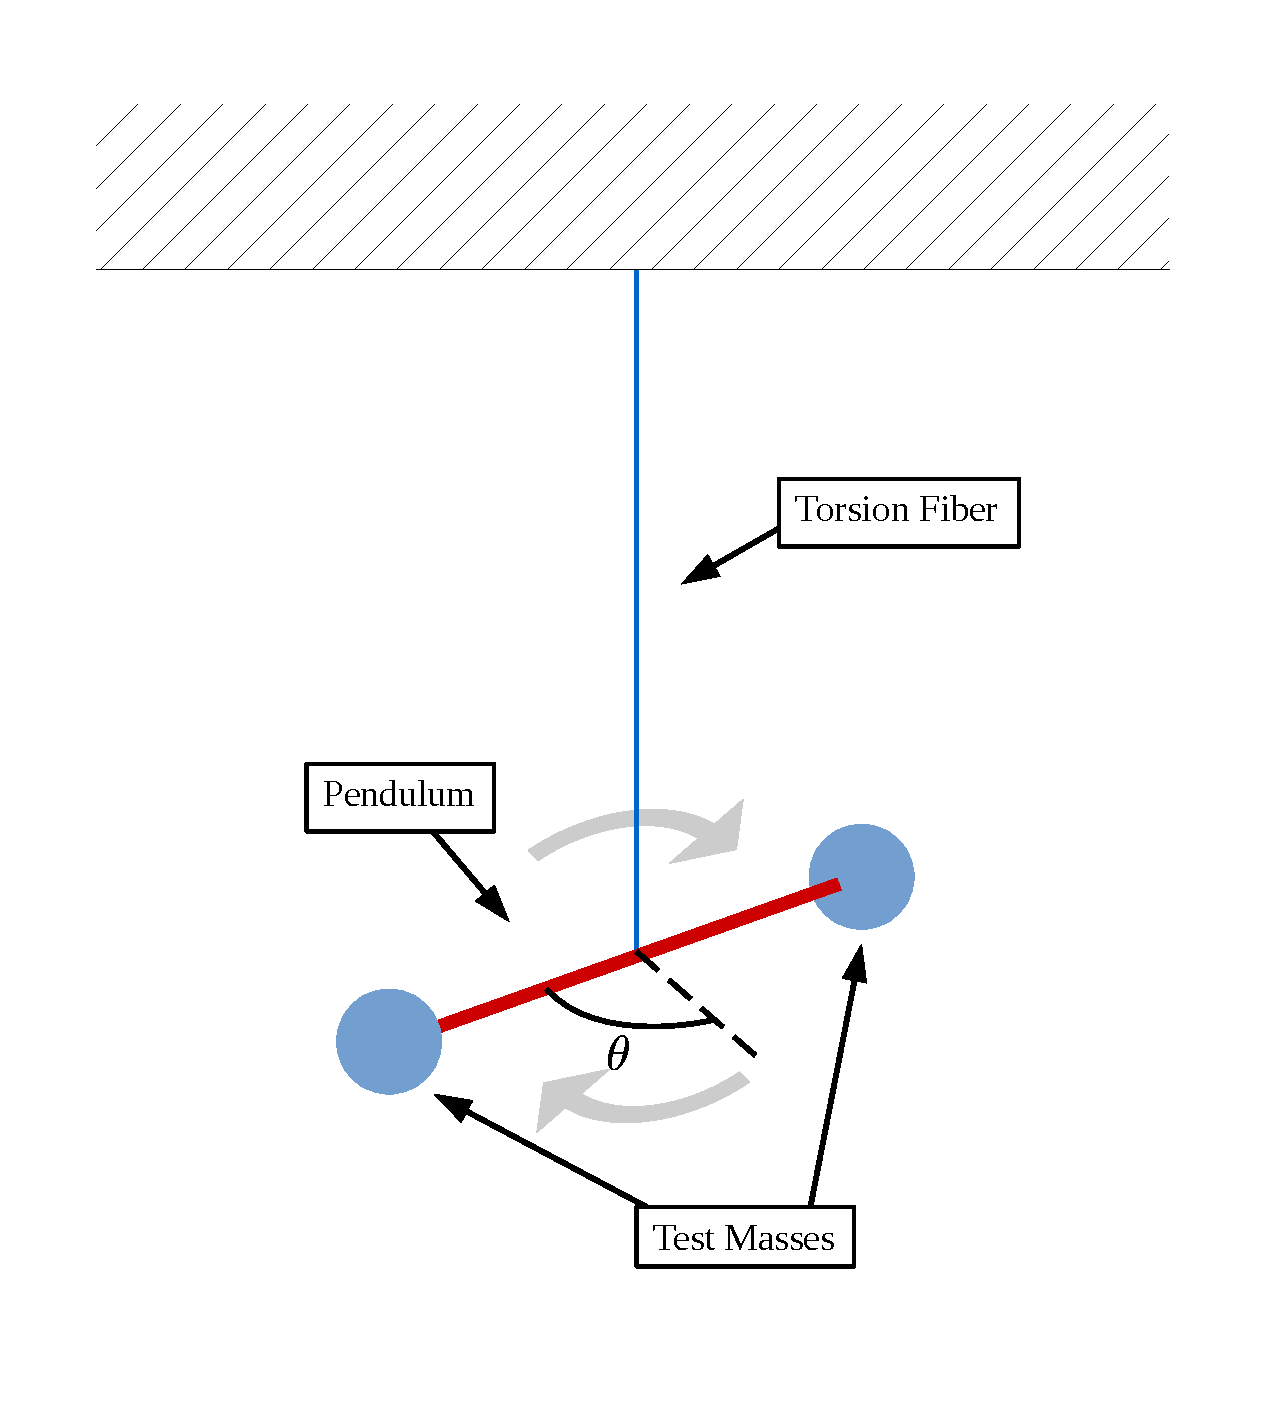
\includegraphics[width=0.65\textwidth]{SimpleTorsionBalance.pdf}
\caption{A simple torsion balance system.}\label{simpleFig}
\end{centering}
\end{figure}

From Hooke's law, the torsional spring adds a restoring torque that follows:
\begin{equation}
\tau_{\text{spring}}(t) = -\kappa (\theta(t)-\theta_0)
\end{equation}
where $\theta_0$ is the equilibrium angle of the torsion balance. For most situations this is the dominant torque acting on the pendulum.

Due to historical reasons, the classical example of a torsion balance is a dumb-bell shaped pendulum suspended from a thin metal fiber, shown in Figure~\ref{simpleFig}. The pendulum is formed by a massless rod with two equal mass "test masses" attached to each end. The torsion fiber is then attached to the rod at equal distance to each test mass. This provides a prototypical model of a torsion balance which we will analyze in detail. Modern torsional balance apparatus typically have pendulums with more complex geometry and may have multiple suspension stages. 

\section{Loss Terms}

\quad There are two primary sources of loss in torsion balances: external and internal damping. External damping, sometimes called velocity damping, is caused by external forces acting on the pendulum that are proportional to the angular velocity of the pendulum, such as air friction. Internal damping, on the other hand, is caused by energy dissipation internal to the torsion fiber.

External damping adds a torque on the pendulum that is proportional to the angular velocity of the pendulum:
\begin{equation}
\tau_{\text{vel}}(t) = -\gamma \dot{\theta}(t)
\end{equation}
where $\gamma$ is the damping constant. Where as internal damping can be modeled by a complex spring constant:
\begin{equation}
\tau_{\text{spring}}(t) =  -\kappa(1+i\delta) \big(\theta(t)-\theta_0\big)
\end{equation}
where $\delta$ is the dimensionless internal loss parameter.

For most modern torsion balances, external damping is engineered away and is thus much smaller than the internal damping. Thus we will shelve discussion of external damping until Section \ref{gas}

\section{Equations of Motion}

\quad As mentioned in Section~\ref{simple}, the simple torsion balance is described with two primary parameters: the moment of inertia, $I$, which is determined by the pendulum geometry, and the torsional spring constant, $\kappa$, which is determined by the torsion fiber size and material. Adding in internal damping, this system obeys the following equation of motion:
\begin{equation}
I~\ddot{\theta}(t)+\kappa(1+i\delta)  \big(\theta(t)-\theta_0\big) = \tau_{\text{ext}}(t) \label{eom}
\end{equation}
where $\tau_{\text{ext}}(t)$ is the sum of all exterior torques acting on the pendulum.

If we assume a harmonic solution, $\theta(t)=A~e^{i\omega t}$, we can transform Equation~\ref{eom} into the Fourier domain to yield:
\begin{equation}
\big(-I\omega^2+\kappa(1+i\delta) \big) \tilde{\theta}(\omega)= \tau_{\text{ext}}(\omega) \label{four}
\end{equation}
It is convenient to define two parameters here: the resonant frequency, $\omega_0=\sqrt{\kappa/I}$, and the quality factor, $Q=\frac{1}{\delta}$. Equation \ref{four} can then be rearranged to:

\begin{equation}
 \tilde{\theta}(\omega)= \frac{\tau_{\text{ext}}(\omega)}{\kappa}\frac{1}{1-\omega^2/\omega_0^2 +i/Q} \label{four2}
\end{equation}

\section{Response Function}\label{resp}

\quad The second dimensionless factor in Equation \ref{four2} is traditionally called the response function or transfer function of the system. It controls the amount of angle the pendulum gets for a given torque as a function of frequency. 

\begin{equation}
\Lambda(\omega)= \frac{1}{1-\omega^2/\omega_0^2 +i/Q} \label{four3}
\end{equation}

For a pendulum with no damping, $Q\rightarrow\infty$, the response function has three distinct features. Below the resonant frequency, $\omega << \omega_0$, the response goes to unity. Above the resonant frequency, $\omega >> \omega_0$, the response function follows $\Lambda(\omega)=-\omega_0^2/\omega^2$ causing effect of high frequency torques to decrease as $1/\omega^2$. At the resonant frequency, $\omega=\omega_0$ the response goes to infinity. This causes the motion at this frequency to grow without limit.

With damping, the response has a similar structure albeit with different amplitudes. Namely at the resonance the response does not approach infinity but instead $\Lambda(\omega)=-i Q$. The quality factor, hence the amount of damping, limits the maximum resonant motion for a given input torque. 

\begin{figure}[!h]
\begin{centering}
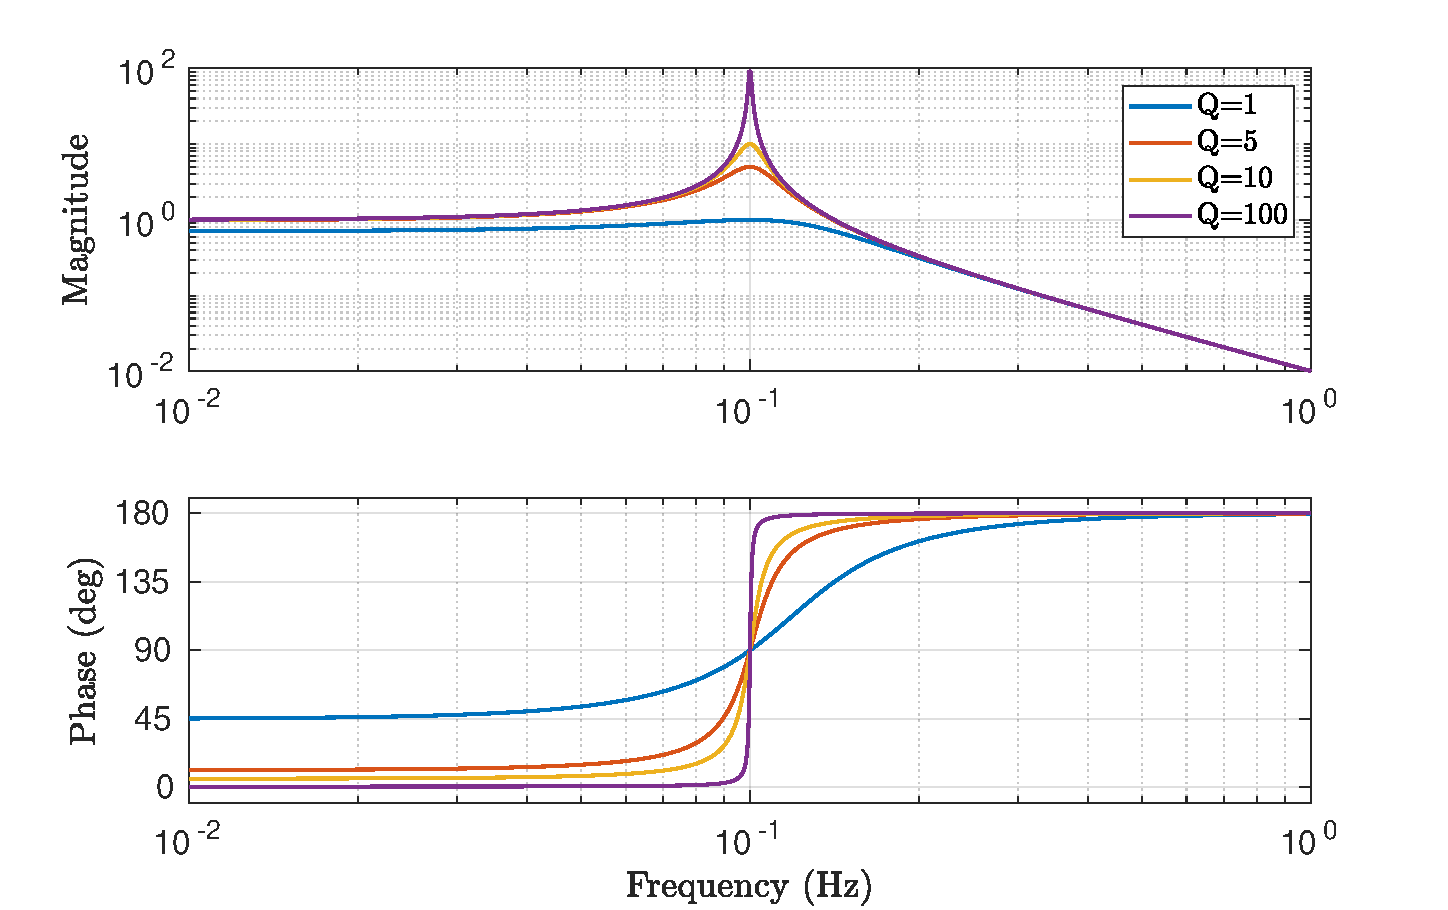
\includegraphics[width=\textwidth]{ResponseFunction.pdf}
\caption{The response function for a simple torsion balance system with a resonance of $\omega_0=2\pi\ (0.1 \text{ Hz})$.}\label{respPlot}
\end{centering}
\end{figure}

The full response function is plotted in Figure \ref{respPlot} for a variety of quality factors and a resonant frequency of 0.1 Hz. As can be seen, below the resonance the magnitude of the response approaches unity with a nearly zero phase for most values of $Q$. There's a peak at the resonant frequency whose amplitude is strongly dependent on $Q$ and the phase undergoes a rapid transition. Above the resonance the magnitude follows $\sim1/\omega^2$ with a phase of $180^\circ$ independent of $Q$-value. Note that a phase of $180^\circ$ is equivalent to a negative sign.


\chapter{Mechanics}
\section{Torque Sensing}

\quad For many experiments, the primary use of a torsion balance is to sense weak torques acting on the pendulum. In this mode, the measurements of the angle of the pendulum is converted to torque by rearranging Equation \ref{four2}:
\begin{equation}
\tau_{\text{ext}} (\omega)= \frac{\kappa\ \tilde{\theta}(\omega)}{\Lambda(\omega)} \label{torq}
\end{equation}

If we assume a frequency-independent angle spectrum, $\tilde{\theta}(\omega)$, (which is unrealistic but a rough approximation of spectra arising from readout noise, Section \ref{readout}) then the corresponding torque spectrum will follow the inverse of the pendulum response function, $\Lambda(\omega)$. An example of such a spectrum is shown in Figure \ref{torqSpec}. This spectrum has very similar features as the response discussed in Section \ref{resp}. However, instead of having a peak at the resonant frequency it has a dip and above the resonant frequency the torque spectrum rises as $\sim \omega^2$. 

These features are the first example we've seen that expresses the significance of the frequency of signal of interest in designing an experiment. A careful experimenter would design an apparatus to minimize the noise at the frequency of interest within practical limits. For example, the model apparatus described by Figure \ref{torqSpec} would not be ideal to run an experiment with a signal at 1 Hz but would be well suited for a signal at 10 mHz since the noise level differs by a factor of 100 between these two frequencies. This is a common consideration in torsion balance design that will reoccur throughout this work.

\begin{figure}[!h]
\begin{centering}
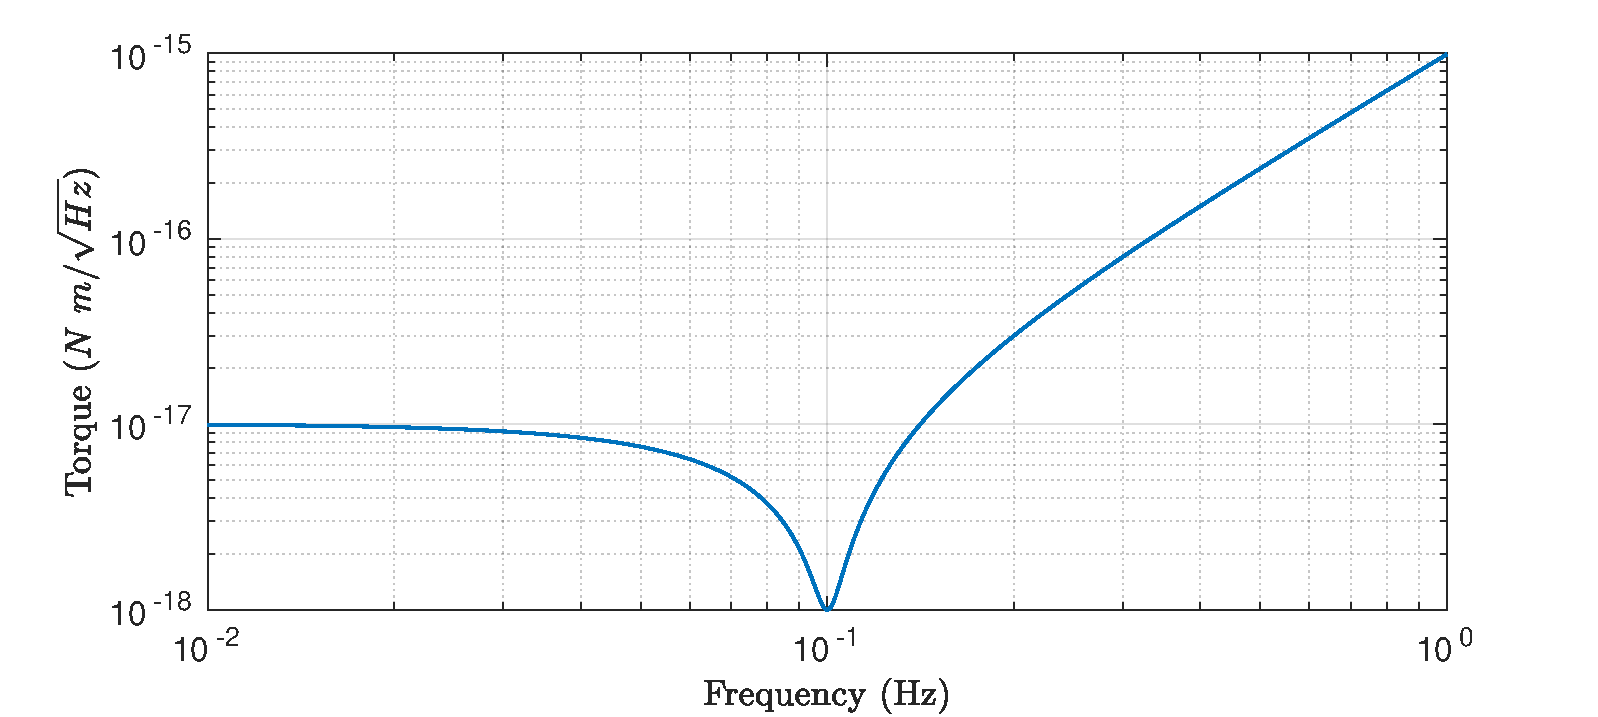
\includegraphics[width=\textwidth]{TorqueSpectrum.pdf}
\caption{Example torque spectrum assuming a frequency independent angle spectrum $\tilde{\theta}(\omega) = 1\ \text{nrad}/\sqrt{\text{Hz}}$ amplitude, $\kappa=10^{-8}\ \text{N m/rad}$, $Q=10$, and $\omega_0=2\pi\ (0.1 \text{ Hz})$ .}\label{torqSpec}
\end{centering}
\end{figure}
\pagebreak
\section{Inertial Sensing}\label{inertSection}

\quad A relatively newer use of torsion balances is for inertial sensing. Where as in the previous section we discussed torques acting on the pendulum, for inertial sensing the pendulum acts as an inertial proof mass. The goal of this mode is to measure the angular motion of structure that the pendulum is suspended from. These sorts of measurements have a wide range of application, from rotational seismology and seismic isolation to guidance systems and navigation. 

A system whose support structure is allowed to move can be modeled with Equation \ref{eom} by allowing $\theta_0$ to vary in time:

\begin{equation}
I~\ddot{\theta}(t)+\kappa(1+i\delta)  \big(\theta(t)-\theta_0(t)\big) = \tau_{\text{ext}}(t) \label{inert}
\end{equation}

Since the motion of the support is what we want to measure, Equation \ref{inert} can be transformed in the Fourier domain and rearranged to yield:

\begin{equation}
\tilde{\theta}(\omega)=\frac{1+i/Q}{1-\omega^2/\omega_0^2+i/Q}\ \tilde{\theta_0}(\omega) \label{inert2}
\end{equation}

However, angular readout systems do not sense the inertial angle of the pendulum but instead measure the difference in angle between the support and the pendulum. (In all other sections we assume the support is inertial.) Thus, the measured angle is:

\begin{equation}
\tilde{\theta_a}(\omega)=\tilde{\theta}(\omega)-\tilde{\theta}_0(\omega) \label{inert3}
\end{equation}

Combining Equations \ref{inert2} and \ref{inert3} yields:

\begin{equation}
\tilde{\theta}_0(\omega)=\frac{\omega_0^2}{\omega^2}\ \frac{1}{\Lambda(\omega)}\ \tilde{\theta}_a(\omega) \label{inert4}
\end{equation}

At first glance, Equation \ref{inert4} looks very similar to the angle response to torque, Equation \ref{four2}. However, the extra factor of $\omega^2/\omega_0^2$ mirrors the features onto opposite sides of the resonance. For a frequency independent measured angle spectrum, the inertial angle spectrum will follow $\sim1/\omega^2$ below the resonance while above it flattens to approach the measured angle spectrum. Figure \ref{inertSpec} shows an example of such a spectrum which displays the same features as Figure \ref{torqSpec} but mirrored about the resonance frequency.

\begin{figure}[!h]
\begin{centering}
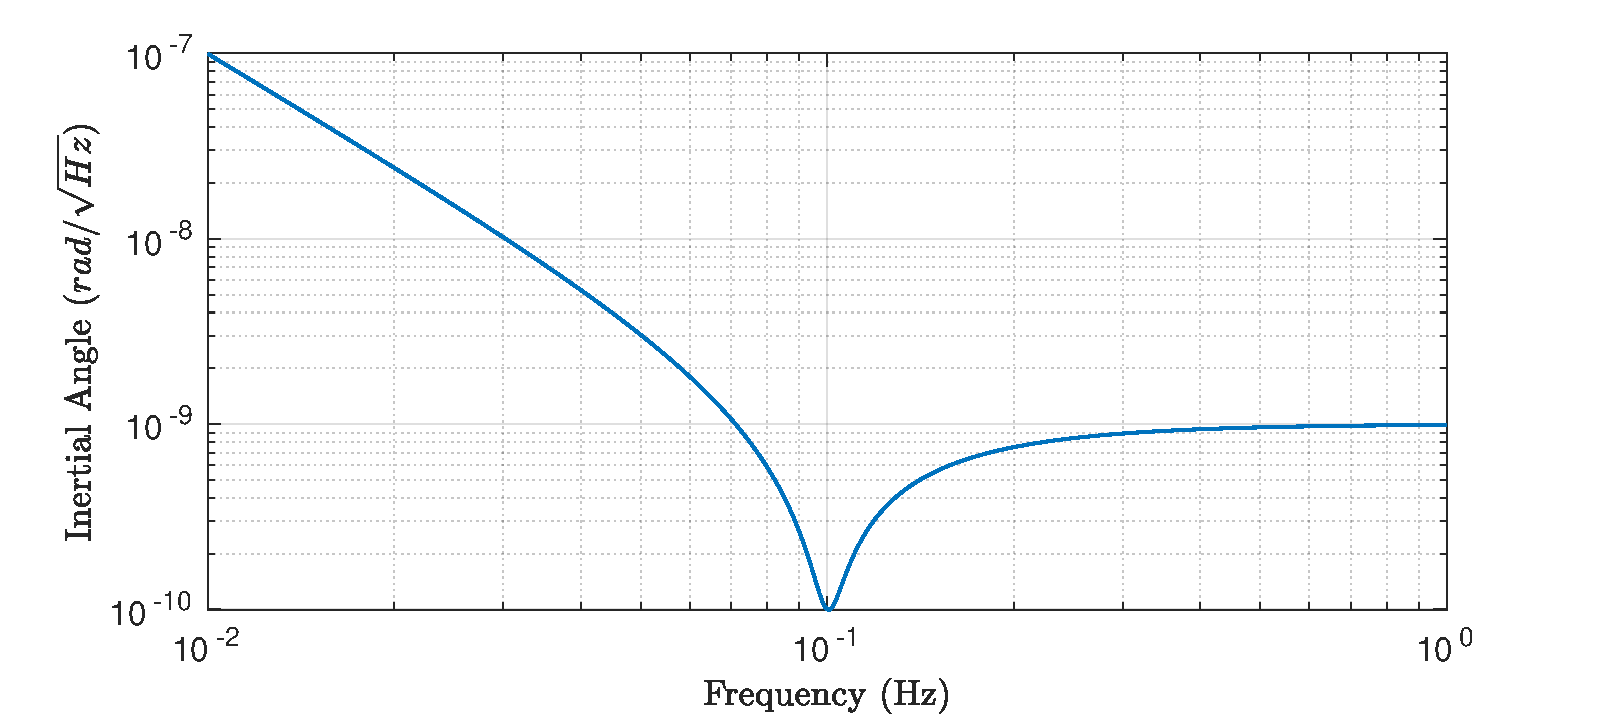
\includegraphics[width=\textwidth]{InertialSpectrum.pdf}
\caption{Example inertial angle spectrum assuming a frequency independent measured angle spectrum $\tilde{\theta_a}(\omega) = 1\ \text{nrad}/\sqrt{\text{Hz}}$ amplitude, $Q=10$, and $\omega_0=2\pi\ (0.1 \text{ Hz})$.}\label{inertSpec}
\end{centering}
\end{figure}

Due to the features of Equation \ref{inert4}, an inertial sensing apparatus achieves its best performance above the resonant frequency and quickly looses sensitively below it. Thus lowering the resonant frequency increases the band of interest.

\section{Fiber Engineering} \label{fiber}

\quad Although it is easy to think of the torsion fiber as a minor part of the torsion balance system, manufacturing the optimal fiber for a given experiment is an art in itself. There are two primary optimizations when designing a torsion fiber: minimizing the $\kappa$ of the fiber and maximizing the $Q$. These are not necessarily orthogonal and many design alterations will drastically change both parameters. 

There is generally three parameters that can be adjusted in a fiber design: the length of the fiber, $l$, the cross-sectional radius\footnote{Here we're assuming a circular cross-section but many fibers have more complex geometries which must be accounted for.}, $r$, and the material. To optimize these parameters, one usually uses the following procedure. First, find out the maximum length that can fit in the given apparatus and use that length of fiber. Then choose a material based on the requirements of the experiment, what is readily available to purchase or manufacture, and which material will give the highest $Q$. Then minimize the fiber radius until the weight of the pendulum is close to the breaking strength of the fiber (with a healthy safety factor to minimize break-ability). This can be iterated through multiple times along with various apparatus changes (chamber height, charge mitigation, etc.) to achieve a near optimal set-up. 

Experimenter's are not left to blindly search for optimal parameters but are instead informed by vast troves of theoretical and experimental information much of which was produced by the engineering communities. The $\kappa$-value for a fiber with uniform cross-section can be readily calculated using \cite{hibbeler2003mechanics}:
\begin{equation}
\kappa = \mu \frac{J}{l} 
\end{equation}
where $\mu$ is the shear modulus of the material, $J$ is the torsional constant of the material, and $l$ is the length of the fiber. The shear modulus depends on the material and temperature whereas the torsional constant only depends on the cross-sectional geometry of the fiber. Assuming a circular cross-section this becomes:
\begin{equation}
\kappa = \mu \frac{\pi r^4}{2 l} \label{kappa}
\end{equation}
where $r$ is the cross-sectional radius of the fiber. Equation \ref{kappa} shows the drastic dependence of $\kappa$ on the radius of the fiber and to a lesser extent the length. The value of the shear modulus, $\mu$, for a given material is typically looked-up in various engineering references. Table \ref{ShearTable} gives the values for a selection of materials typically used in torsion balance apparatus.

\begin{center}		
	\begingroup
	\setlength{\tabcolsep}{10pt} % Default value: 6pt
	\renewcommand{\arraystretch}{1.5} % Default value: 1
	\begin{table}[ht!]
		\begin{center}
			\begin{tabular}{ |c|c| }
				\hline
				Material & Shear Modulus, $\mu$ (GPa) \\
				\hline
				Beryllium Copper (Be-Cu) & 48\\
				Aluminum (Al), 6061-T6 & 224\\
				Tungsten (W) & 161 \\ 
				Titanium (Ti) & 41\\
				Steel & 75\\
				Fused Silica (SiO$_2$) & 31 \\
				\hline
				
			\end{tabular}
			\caption{Table of the shear modulus for a selection of typical materials \cite{shear, quartz}.}\label{ShearTable}
		\end{center}
	\end{table}
	\endgroup
\end{center}

Naively, Equation \ref{kappa} could be interpreted as allowing arbitrarily low $\kappa$-values since up to this point we have not set any limits on the minimum width of the torsion fiber. However, in addition to providing the restoring torque, the fiber must also hold the pendulum's weight. The maximum force that a fiber can experience without deforming\footnote{There are two tensile strengths one could use: the yield strength or the ultimate tensile strength. The yield strength is the point at which the material deforms while the ultimate tensile strength is when it breaks. The ultimate tensile strength is typically less than twice the yield strength. Here we use the yield strength as it is lower than the ultimate tensile strength and deformation of a torsion fiber would alter the other parameters discussed here.} follows:
\begin{equation}
F=\sigma \pi r^2
\end{equation}
where $\sigma$ is the yield strength of the material and $r$ is the cross-sectional radius. The minimum radius needed to hold a pendulum is then:
\begin{equation}
r_{\text{min}}=\sqrt{\frac{m g}{\pi \sigma}}
\end{equation}
where $m$ is the mass of the pendulum and $g$ is the local gravitational acceleration. A fiber of this radius could hold the pendulum but any further force (earthquake, anthropogenic forces, etc.) on the fiber would cause it to yield. Thus a safety factor is used to ensure the apparatus is robust against laboratory conditions.
\begin{equation}
r_{\text{safe}}=\eta \sqrt{\frac{m g}{\pi \sigma}}
\end{equation}
where $\eta$ is the safety factor with typical values in the range of 2 - 3. Yield strength is another parameter which in practice is looked-up in engineering references. Table \ref{YieldTable} shows values for a collection of typical materials used for torsion fibers.

\begin{center}		
	\begingroup
	\setlength{\tabcolsep}{10pt} % Default value: 6pt
	\renewcommand{\arraystretch}{1.5} % Default value: 1
	\begin{table}[ht!]
		\begin{center}
			\begin{tabular}{ |c|c| }
				\hline
				Material & Yield Strength, $\sigma$ (MPa) \\
				\hline
				Beryllium Copper (Be-Cu) & 965 - 1205 \\
				Aluminum (Al), 6061-T6 & 241\\
				Tungsten (W) & 550 \\ 
				Titanium (Ti) & 100 - 225\\
				Steel & 75\\
				Fused Silica (SiO$_2$) & 48\\
				\hline
				
			\end{tabular}
			\caption{Table of yield strengths for a selection of typical materials \cite{quartz, yield, alum, becu}.}\label{YieldTable}
		\end{center}
	\end{table}
	\endgroup
\end{center}

The quality factor, $Q$, is also an important consideration when engineering a torsion fiber. The $Q$-value is inversely proportional to the amount of mechanical energy dissipated in the fiber. Thus, the $Q$-value not only changes the response function of the system, as can be seen in Figure \ref{respPlot}, but also influences the amount of thermal noise in the system. Thermal noise is discussed in detail in Section \ref{thermal}; however when it comes to fiber design the important fact is that thermal torque noise follows, $\tau \sim 1/\sqrt{Q}$. Thus the higher the $Q$ the lower the thermal noise.

The exact value of the quality factor of a given fiber is dependent on a variety of factors, from the mechanics of the end points to the presence of surface defects. However, many materials are known to have larger $Q$-values than others. Generally, if the material is more uniform then it will have a larger $Q$-value. Metals are the traditional choice especially those historically used in musical instruments (bells, guitar strings, etc.). Specifically, tungsten fibers are known to achieve $Q$-values of $\sim4500$ \cite{qual}. A type of glass called fused silica or fused quartz is also well known to be a high-$Q$ material. It is formed from almost pure silicon dioxide (SiO$_2$) and can achieve $Q$-values as high as $10^5$ \cite{qual}. As compared to metals, fused silica is extremely delicate and thus many hours of lab work can be ruined by simply touching the fiber. To many experimenter's, including those at the world's gravitational wave observatories, this risk is well worth the exceedingly high $Q$-values achieved by this material.

\section{Pendulum Design}

\quad Engineering a suitable fiber doesn't in itself make for a high-quality torsion balance; a quality pendulum is the other key ingredient. Much of the pendulum design depends strongly on the experiment that is to be conducted with the apparatus. Yet there are a few common guidelines that lead to the top performing pendulums. 

With every pendulum, there is mass that is used in the scientific experiment, which we call active mass, and mass that only serves as structural support, called passive mass. In the simple torsion pendulum shown in Figure \ref{simpleFig}, the active mass would be the test-masses while the passive would be the rod. Since many experiments are more sensitive if the apparatus has more active mass, experimenter's want to maximize the active mass and minimize the passive. The figure of merit for a given pendulum design is the ratio of the active mass and the total mass:

\begin{equation}
\alpha = \frac{m_{\text{active}}}{m_{\text{active}}+m_{\text{passive}}}
\end{equation}

Ideally, $\alpha=1$ (such as in the massless-rod, simple pendulum example) which would imply that all of the mass of the pendulum is participating in the experiment. However, no realistic pendulum achieves this and $\alpha$-values of 40-60\% are considered satisfactory.

The other parameter that is directly controlled by the pendulum design is the moment of inertia, $I$. The moment of inertia can be calculated via:
\begin{equation}
I=\int \rho(\vec{r})\ r^2\ dV
\end{equation}
where $\vec{r}$ is the vector from the rotation axis to a point in the pendulum, $\rho$ is the mass density at that point, and $dV$ is the corresponding volume element. This integral is taken over the entire volume of the pendulum.
If we align the $z$-axis with the torsion fiber then the torsional moment inertia\footnote{There is a different moment of inertia for each rotation axis. Here we only calculate the torsional moment (i.e. for rotations around the $z$-axis) but a similar procedure can yield the other moments. Generally, there's a moment of inertia tensor which allows one to calculate the moment around any axis of rotation.} can be found with:
\begin{equation}
I=\int \rho(x,y,z)\ (x^2+y^2)\ dx\ dy\ dz
\end{equation}

For the simple torsion balance described in Section \ref{simple} the mass density is simply Dirac delta functions which follow (aligning the $x$-axis with the pendulum rod):
\begin{equation}
\rho(x,y,z)  = m\ \delta(x^2-R^2)\ \delta(y)\ \delta(z)
\end{equation}
where $m$ is the mass of one test mass and $R$ is the ``lever-arm'' (the radius from the torsion fiber to the test masses). The moment of inertia then simplifies to:
\begin{equation}
I=2 m R^2 \label{inert}
\end{equation}

Although Equation \ref{inert} is for an idealized pendulum, moments of inertia for realistic geometries follow the same scaling (i.e. $I\sim mR^2$). The primary effect of the moment of inertia on the equation of motion is the change of the resonant frequency:
\begin{equation}
\omega_0=\sqrt{\frac{\kappa}{I}}\sim \frac{1}{R} \sqrt{\frac{\kappa}{m}}
\end{equation}

The lever-arm not only affects the moment of inertia but can also influence the sensitivity of a given experiment. If the experiment is searching for a new force, $\vec{F}_\text{new}$, then the torque experienced by the pendulum will follow:
\begin{equation}
\tau(t)=\vec{r} \times \vec{F}_\text{new}\sim R\ F_\text{new}
\end{equation}
Thus for a given torque sensitivity, the larger the lever-arm the more sensitive the experiment is to new forces. This is why most experimenters place the test masses at the largest radius allowed in the given apparatus.

In addition to maximizing the active mass and tuning the geometry, a pendulum design must account for a variety of extraneous couplings and noise sources that are addressed in later sections. These include allowing angle readout, Section \ref{readout}, minimizing electrostatic coupling, Section \ref{elect}, and accounting for gravity gradients, Section \ref{gravGrad}. 

\chapter{Complications}
\section{Swing Modes} \label{swing}

\quad Up to this point, we have only focused on the torsional degree of freedom but any torsion balance with a non-zero length torsion fiber will also permit ``swing'' modes. These are the prototypical pendulum modes whose restoring force is due to gravity not the torsion spring. Figure \ref{swingFig} shows the swing degree of freedom for our simple torsion balance system.

\begin{figure}[!h]
\begin{centering}
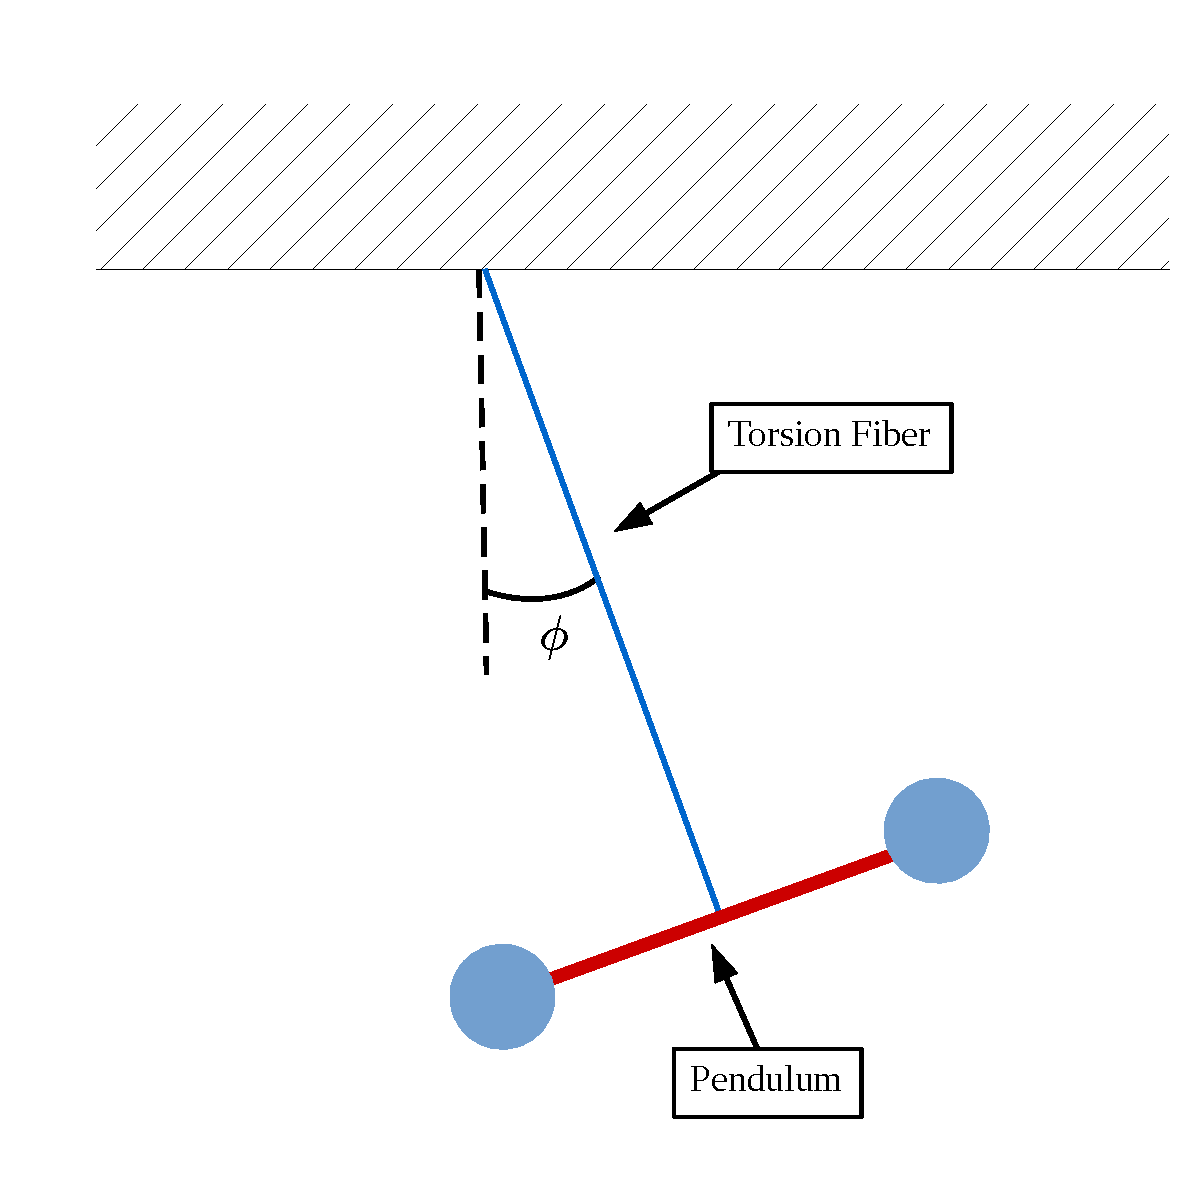
\includegraphics[width=0.65\textwidth]{Swing.pdf}
\caption{The swing degree of freedom for a simple torsion balance system.}\label{swingFig}
\end{centering}
\end{figure}

Restricting ourselves to one swing axis and allowing for external damping of this motion, the equation of motion for the swing degree of freedom is:
\begin{equation}
I_\phi\ \ddot{\phi}(t)+\gamma_\phi \dot{\phi}(t) - \tau_g(t)=\tau_\phi(t)
\end{equation}
where $I_\phi$ is the moment of inertia about the swing axis (into the page in Figure~\ref{swing}), $\phi$ is the swing angle of the pendulum, $\gamma_\phi$ is the swing damping constant, $\tau_g$ is the gravitational restoring torque, and $\tau_\phi$ is the exterior torque about the swing axis. Treating the pendulum as a point mass gives:
\begin{equation}
m l^2 \ddot{\phi}(t)+\gamma_\phi \dot{\phi}(t)+m g l \sin(\phi(t))=\tau_\phi(t)
\end{equation}
where $m$ is the mass of the pendulum, $l$ is the length of the torsion fiber, and $g$ is the local gravitational acceleration. If we take the small-$\phi$ approximation the equation of motion becomes:
\begin{equation}
\ddot{\phi}(t)+\frac{\gamma_\phi}{m l^2} \dot{\phi}(t)+\frac{g}{l} \phi(t)=\frac{\tau_\phi(t)}{m l^2}
\end{equation}
If we define $\nu_0=\sqrt{g/l}$ and $\nu_0/\Omega=\gamma_\phi/(m l^2)$, the equation of motion in the Fourier domain becomes:

\begin{equation}
\phi(\omega)=\frac{\tau_\phi(t)}{m g l} \frac{1}{1-\omega^2/\nu_0^2+i\omega/(\nu_0\Omega)}
\end{equation}


 \begin{figure}[!h]
\begin{centering}
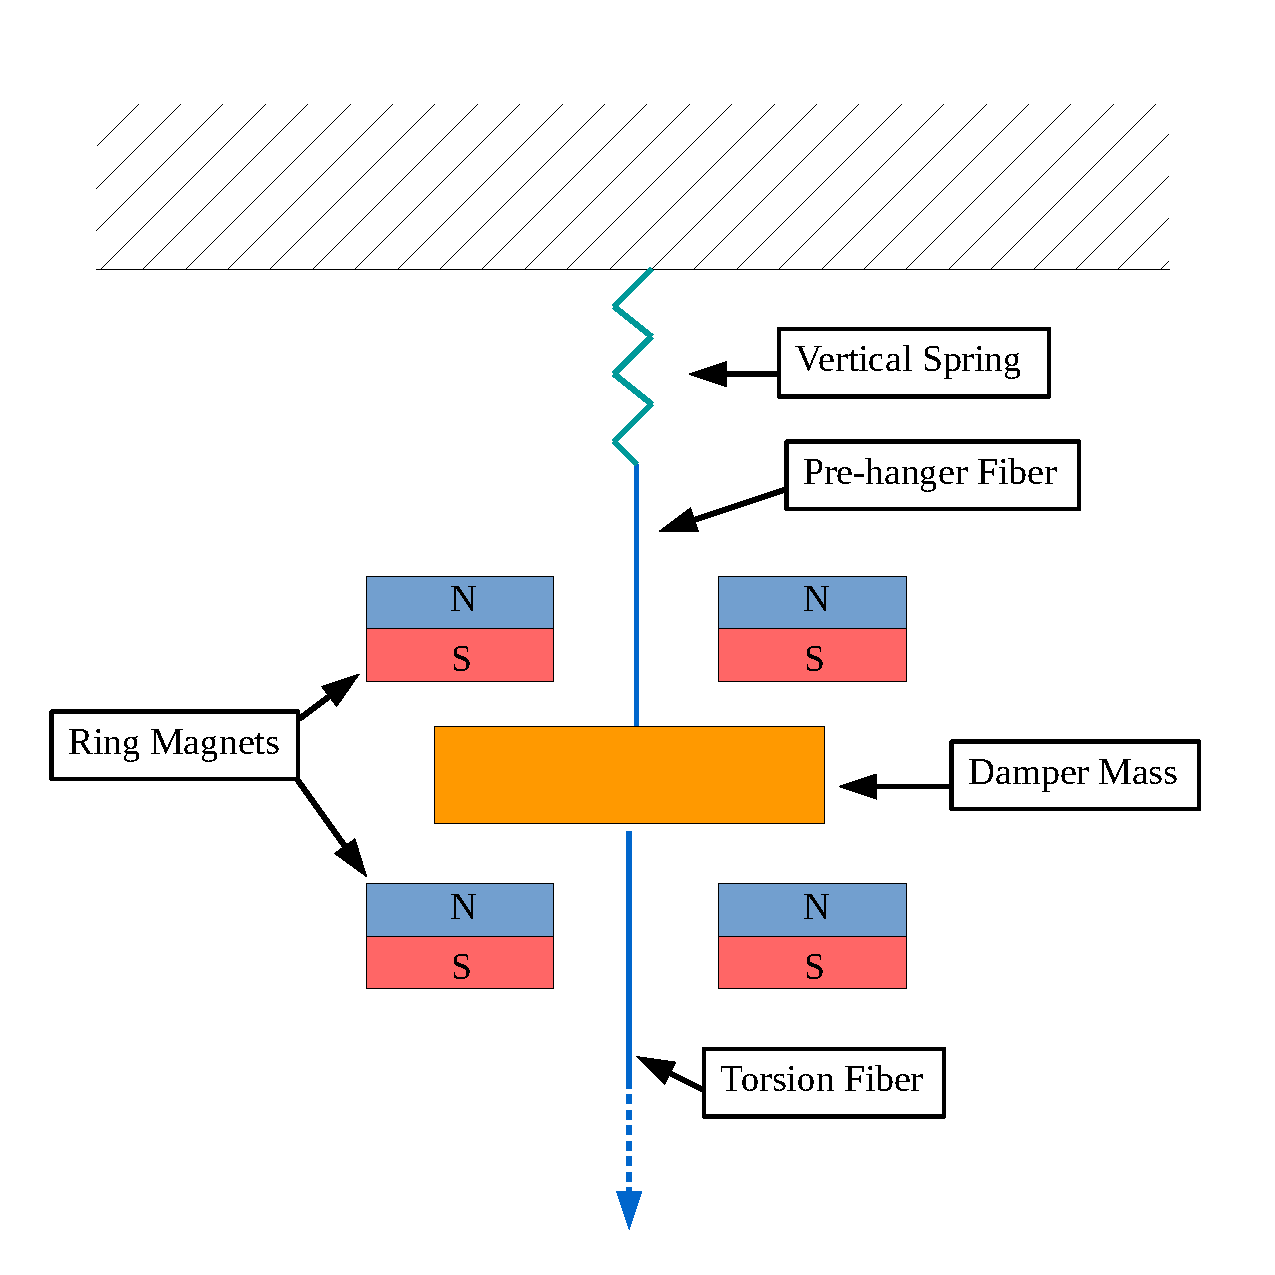
\includegraphics[width=0.65\textwidth]{Damper.pdf}
\caption{Schematic of eddy-current damper.}\label{damper}
\end{centering}
\end{figure}

Excess swing motion can have detrimental effects on the performance of an apparatus. The primary effect of swing motion is addition noise in the torsional degree of freedom. This can be caused by either mechanical cross-coupling converting swing motion into torsional motion or, more commonly, non-linearities in the angular readout systems, Section \ref{readout}, causing swing to register as torsional readings. Thus, any sensitive torsion balance will include some method to limit this swing motion.

The traditional way to limit swing motion is with the addition of an eddy-current swing damper, shown in Figure \ref{damper}. This consists of a conducting damper-mass which is suspended from a pre-hanger fiber and a vertical spring. The torsion balance is then suspended from the damper-mass. The pre-hanger fiber is typically larger diameter than the torsion fiber to separate the double pendulum modes. To achieve eddy-current damping this mass is placed is a non-uniform magnetic field typically produced by a pair of ring magnetics held by an independent structure.

As the damper mass moves in the non-uniform magnetic field, eddy currents are produced in the mass which dissipates the mechanical motion. 

\section{Centrifugal Force}

\begin{figure}[!h]
\begin{centering}
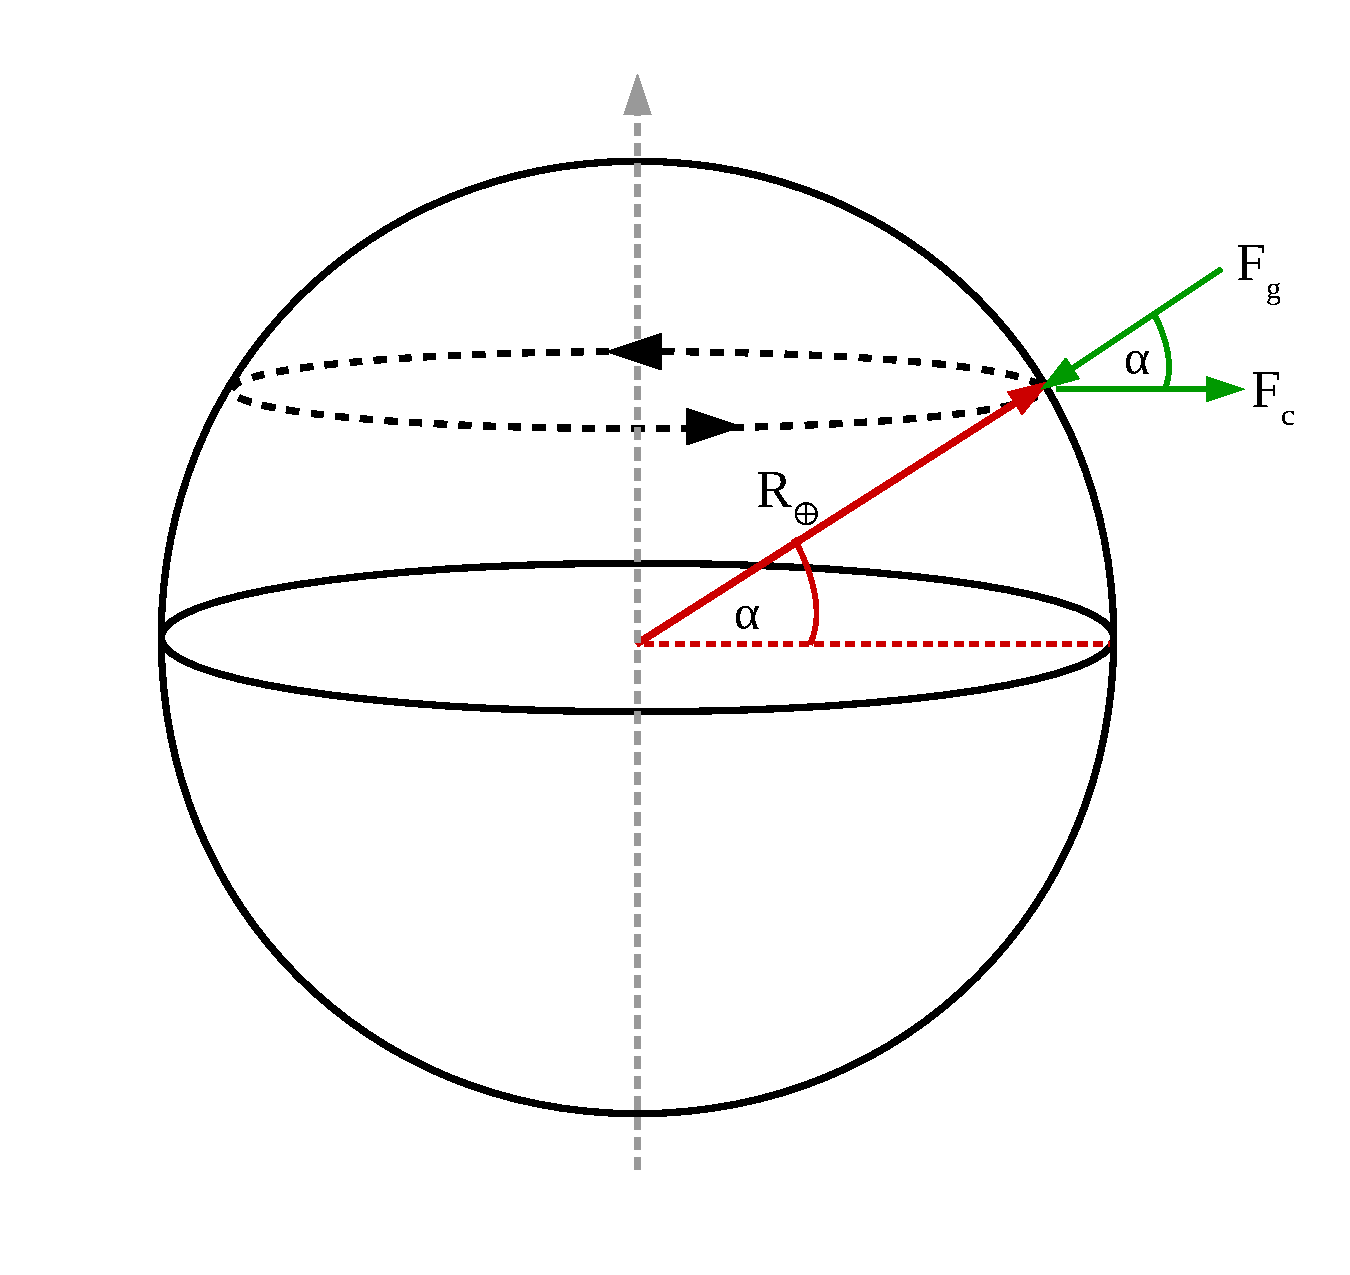
\includegraphics[width=0.45\textwidth]{Centrifugal.pdf}
\caption{Geometry of forces caused by having the torsion balance on the surface of the Earth.}\label{centFig}
\end{centering}
\end{figure}

For most practical purposes, we assume that the torsion fiber runs parallel to local gravity. If the Earth was a perfect sphere the fiber would point directly towards the center of the Earth. However, this is only true if the torsion balance is located at either the equator or one of the planet's poles. Torsion balances experience two forces due to being located on the surface of the Earth: the gravitational pull of the Earth and the centrifugal force due to the Earth's rotation. These together determine the equilibrium swing angle which is not pointed along local gravity.

Since the Earth is rotating, the torsion balance feels a centrifugal force that points perpendicular to the rotation axis of the Earth and follows:
\begin{equation}
F_c= m \omega_\oplus^2R_\oplus \cos \alpha
\end{equation}
where $m$ is the mass of the pendulum, $\omega_\oplus$ is the angular frequency of the Earth, $R_\oplus$ is the radius of the Earth, and $\alpha$ is the latitude of the torsion balance's location. Figure \ref{centFig} shows the geometry of this force along with the gravitational force due to the Earth.


 \begin{figure}[!h]
\begin{centering}
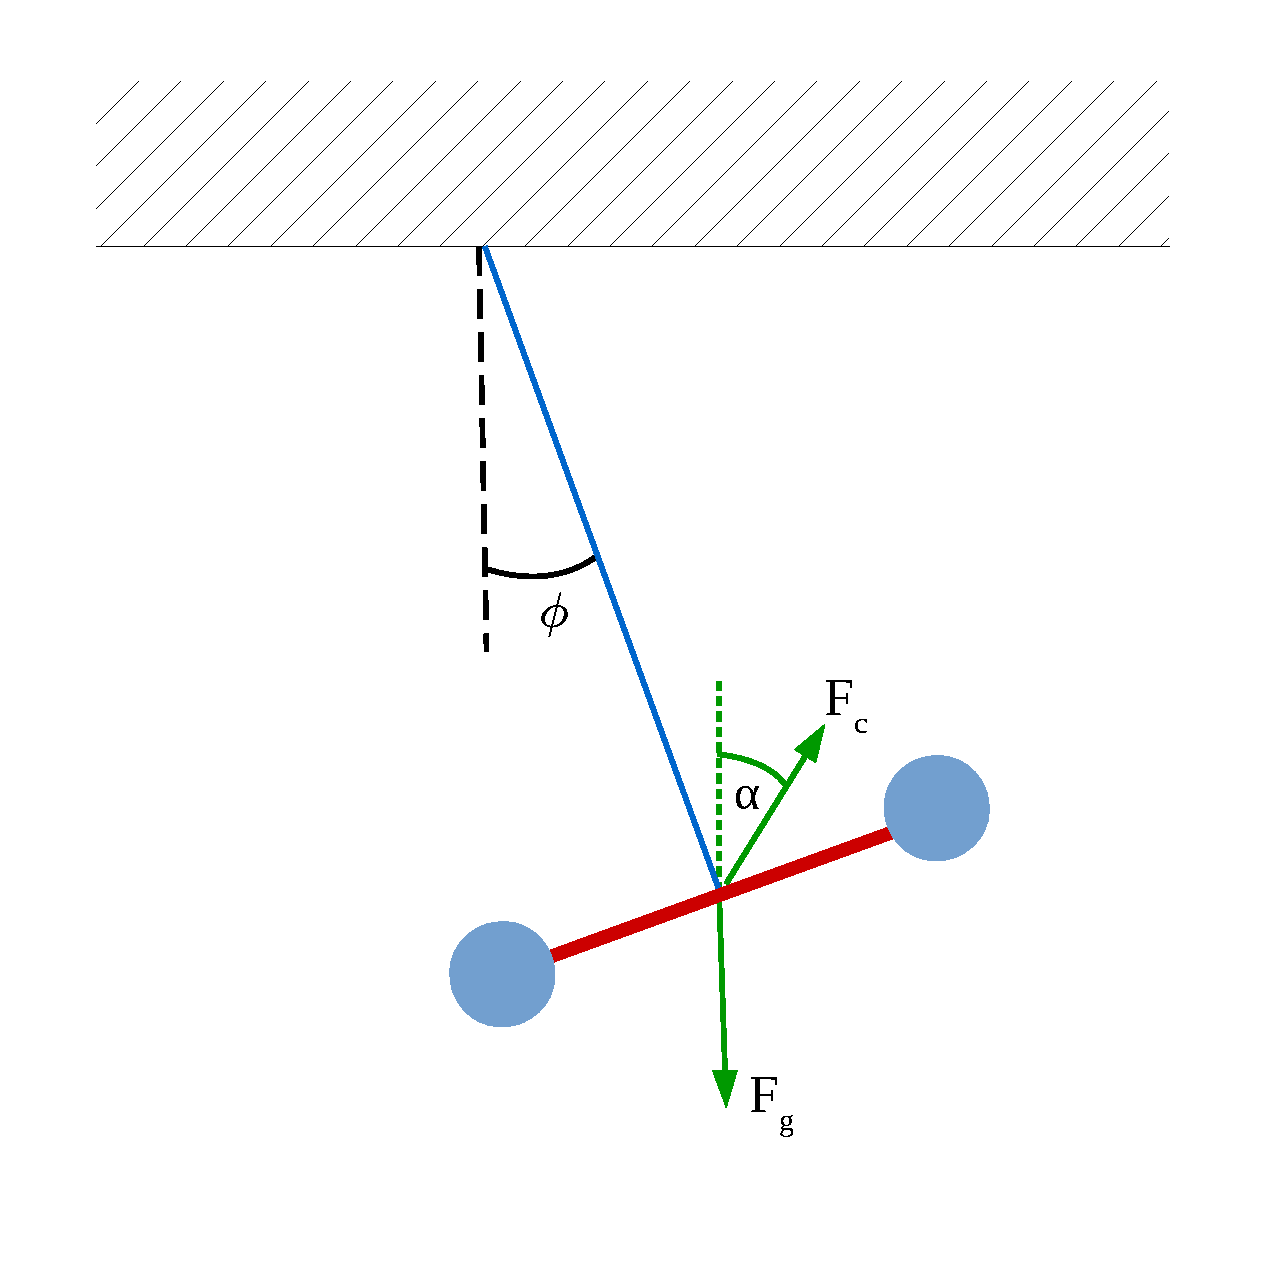
\includegraphics[width=0.65\textwidth]{CentrifugalForce.pdf}
\caption{Force diagram for the forces acting on the torsion balance in equilibrium.}\label{centForFig}
\end{centering}
\end{figure}

In the lab frame, the centrifugal force points upwards at an angle from local vertical equal to the latitude of the torsion balances location as shown in Figure \ref{centForFig}. This provides an additional torque on the balance which shifts its swing equilibrium angle to be:
\begin{equation}
\phi_0 = \arctan\bigg(\frac{\omega_\oplus^2R_\oplus \cos \alpha \sin \alpha}{g-\omega^2R_\oplus \cos^2 \alpha}\bigg) \label{centEq}
\end{equation}

Figure \ref{centPlotFig} shows the Equation \ref{centEq} evaluated at a collection of northern hemisphere latitudes. The southern hemisphere (negative latitudes) has the same magnitude effect but opposite sign. This effect is maximum at 45$^\circ$ latitude at which the pendulum hangs $\sim1.7$ mrad away from local vertical. 

 \begin{figure}[!h]
\begin{centering}
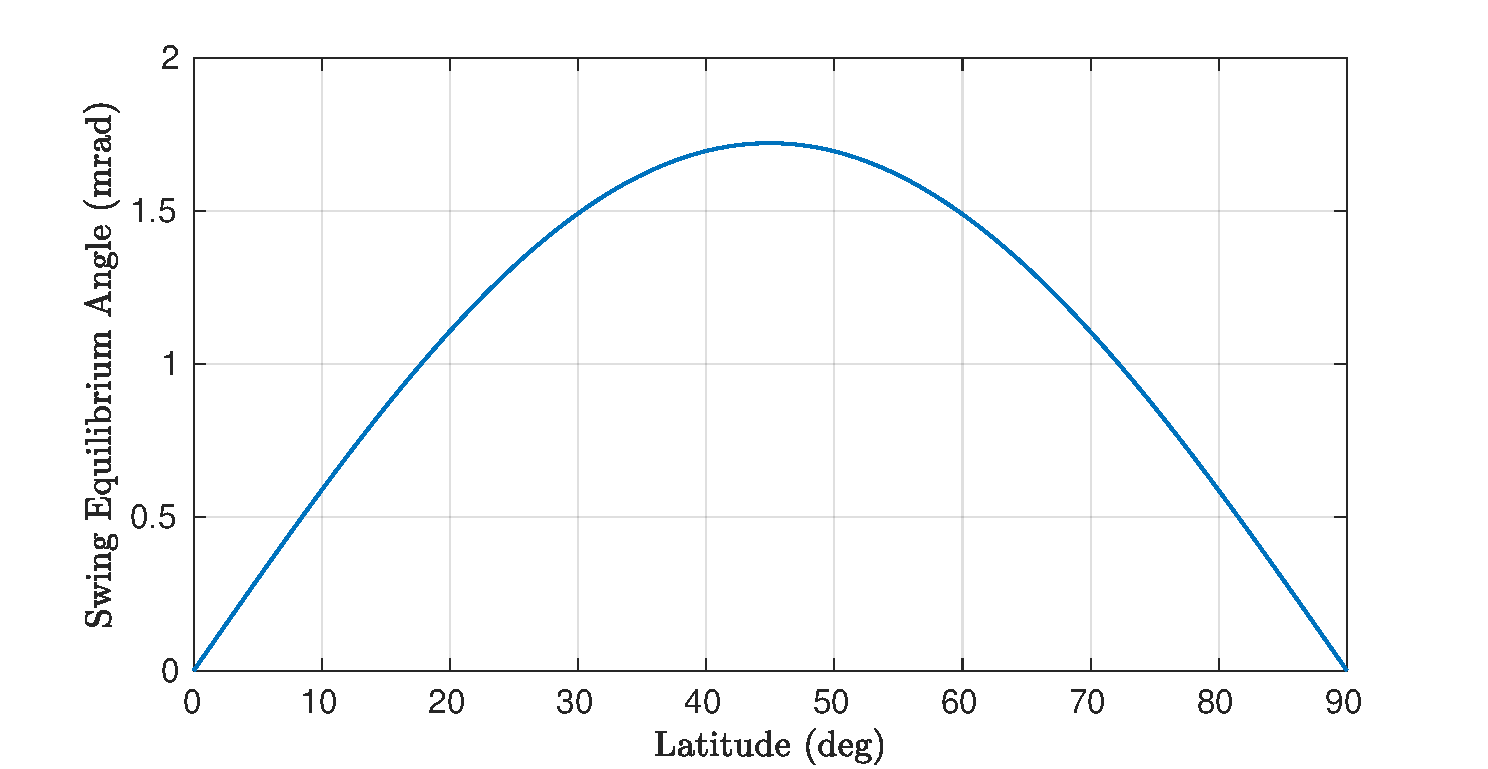
\includegraphics[width=0.85\textwidth]{CentrifugalPlot.pdf}
\caption{Plot of swing equilibrium angle vs. latitude.}\label{centPlotFig}
\end{centering}
\end{figure}

Although this shift has little effect on many experiments, it allows torsion balances to use the Earth as a source mass at most latitudes. This is used in many equivalence principle tests as well as using torsion balances for geophysical exploration.

%\section{Double Pendulum} \label{double}



\chapter{Noise Sources and Mitigation}

\quad Although experimenters try their hardest, torsion pendulums do not exist in the pristine environments we like to cook up on chalkboards. The have a long list of interactions with the universe that end up plaguing experiments. Calling an effect noise verses signal is a choice of viewpoint. Here we will assume the science being conducted is not related to the environment but is instead a novel force or a torque that's controlled by the experimenter. Of course noise can become signal if one was aiming to study one of these effects.

\section{Thermal Noise} \label{thermal}

\quad The fact that torsion balances are at finite temperature causes ever-present ``thermal'' noise which is one of the most difficult to mitigate. There are multiple ways to view this noise source. On a microscopic level, it is caused by the thermal motion of the atoms that make up the torsion fiber. Abstracting a bit more, it is due to application of the fluctuation-dissipation theorem \cite{flucDis} to the torsion balance system.

This thermal motion causes a stochastic torque that follows \cite{thermal}:
\begin{equation}
\tau (\omega)= \sqrt{4 k_B T\bigg( \frac{\kappa}{Q} \bigg) \bigg( \frac{1}{\omega} \bigg)}\label{thermEq}
\end{equation}
where $k_B$ is Boltzman's constant, $T$ is the temperature, $\kappa$ is the spring constant, $Q$ is the quality factor, and $\omega$ is the angular frequency. Note that this torque noise follows $\sim 1/\sqrt{\omega}$ and thus increases in amplitude at lower frequencies. An example thermal noise is plotted in Figure \ref{noiseSpec} along with an example readout noise, Section \ref{readout}.

There are three parameters that can be altered to minimize this noise. For most torsion balances the temperature is set by the ambient temperature of the laboratory; however, a few experimenter's have investigated cooling their apparatus to cryogenic temperatures. The other two, $\kappa$ and $Q$, are determined by the torsion fiber and thus readily engineered. 

We've already seen that minimizing the $\kappa$-value increases a torsion balance's sensitivity to torques but Equation \ref{thermEq} shows an additional benefit of lowering the amplitude of thermal noise. Additionally, maximizing the $Q$-value further decreases the amplitude. Although these techniques can decrease the influence of this noise on a given apparatus, thermal noise can never be completely avoided and limits the performance of many torsion balance apparatus.

\section{Readout Noise}\label{readout}

\quad The angle of the torsion balance needs to be measured in someway. In today's world, this is done almost exclusively with some sort of analog, precision measuring device communicating to a computer through a analog-to-digital converter (ADC). The measuring device can either directly measure the change in angle (autocollimator, optical levers, etc.) or measure the translation of a part of the pendulum (interferometers, capacitors, etc.). 

If the device's native units are translation, then the measurements must be translated into angle using the following:

\begin{equation}
\sin\big(\theta(t)\big)\approx \theta(t)=\frac{x(t)}{a}
\end{equation}
where $x(t)$ is the recorded translation and $a$ is distance from the torsion fiber axis to the measurement point. In order to maximize the sensitivity of the experiment, astute experimenters who deploy such readout schemes place the measurement point as close to the edge of the pendulum as possible\footnote{Yet another place where large lever-arm helps the experiment.}, $a\approx R$. 

The act of 

\begin{figure}[!h]
\begin{centering}
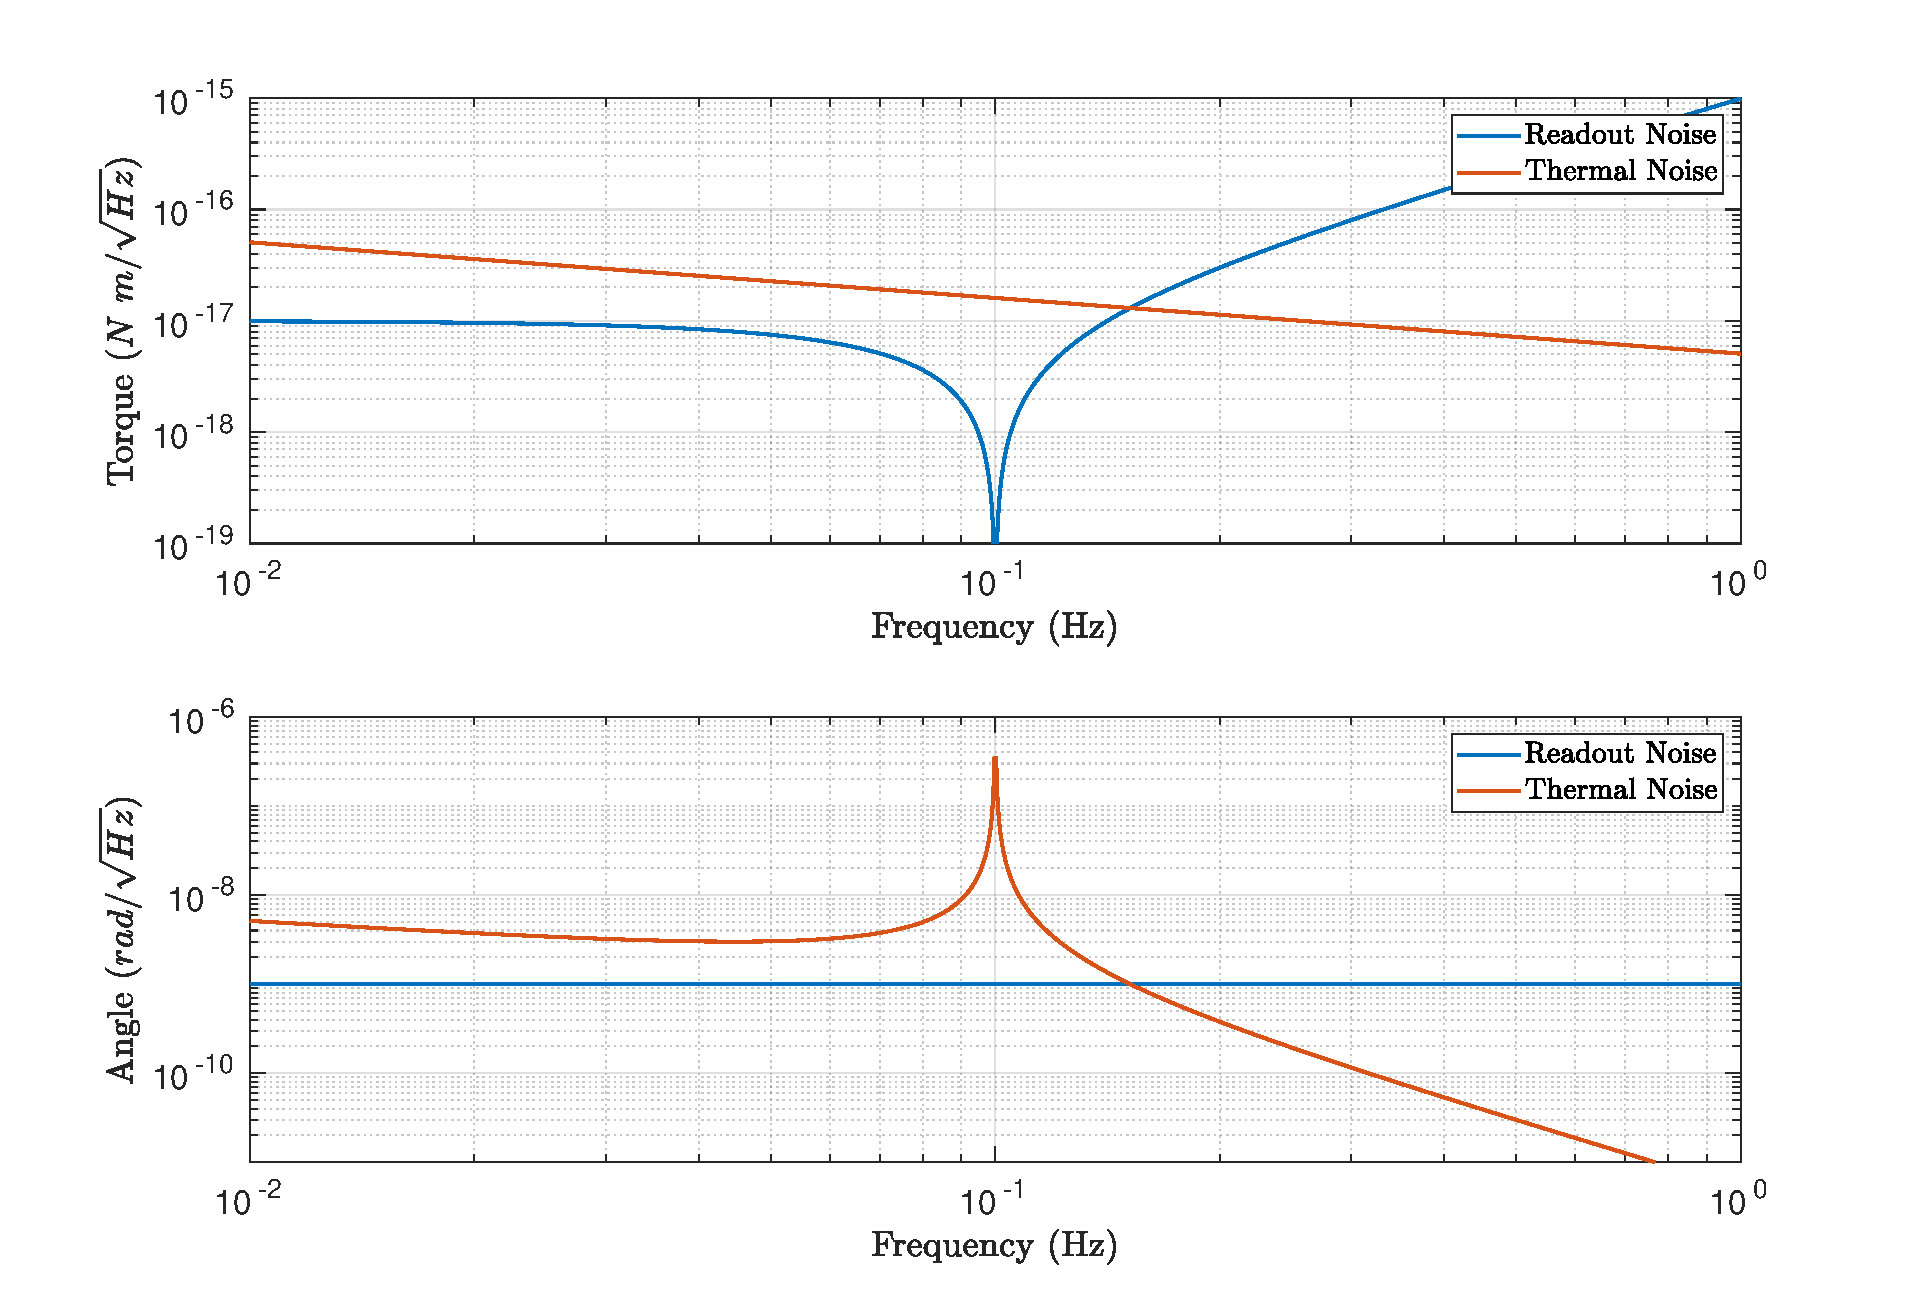
\includegraphics[width=\textwidth]{NoiseSpectrum.pdf}
\caption{Example torque-noise and equivalent angle-noise spectra assuming a readout angle spectrum of $\tilde{\theta}(\omega) = 1\ \text{nrad}/\sqrt{\text{Hz}}$ amplitude, $\kappa=10^{-8}\ \text{N m/rad}$, $Q=10^6$, $T=293\ \text{K}$, and $\omega_0=2\pi\ (0.1 \text{ Hz})$. The total observed noise of such a system would be the sum of the two contributions.}\label{noiseSpec}
\end{centering}
\end{figure}

\section{Seismic Motion}

\quad Even though we don't perceive it in our everyday lives, the ground is always moving. Whether from human activity, the oceans, or the atmosphere, ground motion is constantly being driven. This can be seen in Figure \ref{groundSpec} which displays the amplitude spectral density of typical horizontal seismometer readings \cite{ross2020precision}. Seismometers are spring-mass systems that use the same dynamics as those described in Section \ref{inertSection} to measure ground motion above their resonant frequency. 

Different sources cause motion at distinct frequencies. Above 1 Hz the motion is typically dominated by anthropogenic sources. Whether it's fans from equipment and heating system or vibrations from cars, buses, and trains, human activity causes significant ground motion. This motion typically only appears above 1 Hz due the time scales of most human activity and the dominance of the oceanic microseism at lower frequencies. 

There are persistent, long-wavelength pressure waves within the ocean's water column that are caused by the interference between atmospherically driven surface waves and the ocean floor. These pressure waves drive the dominant persistent ground motion seen everywhere on earth which we called the oceanic microseism (or just microseism for short). The exact amplitude and frequency content of this motion depends on oceanic weather but every seismometer on the surface of the earth senses a broad peak typically between 10 mHz - 1 Hz with peak amplitude of 0.1 - 1 $\mu$m/s/$\sqrt{\text{Hz}}$. At frequencies lower than $\sim$10 mHz, true ground motion is relatively low but seismometer readings become dominated by ground rotations. See Reference \cite{ross2020precision} for more details on ground rotations.

\begin{figure}[!h]
\begin{centering}
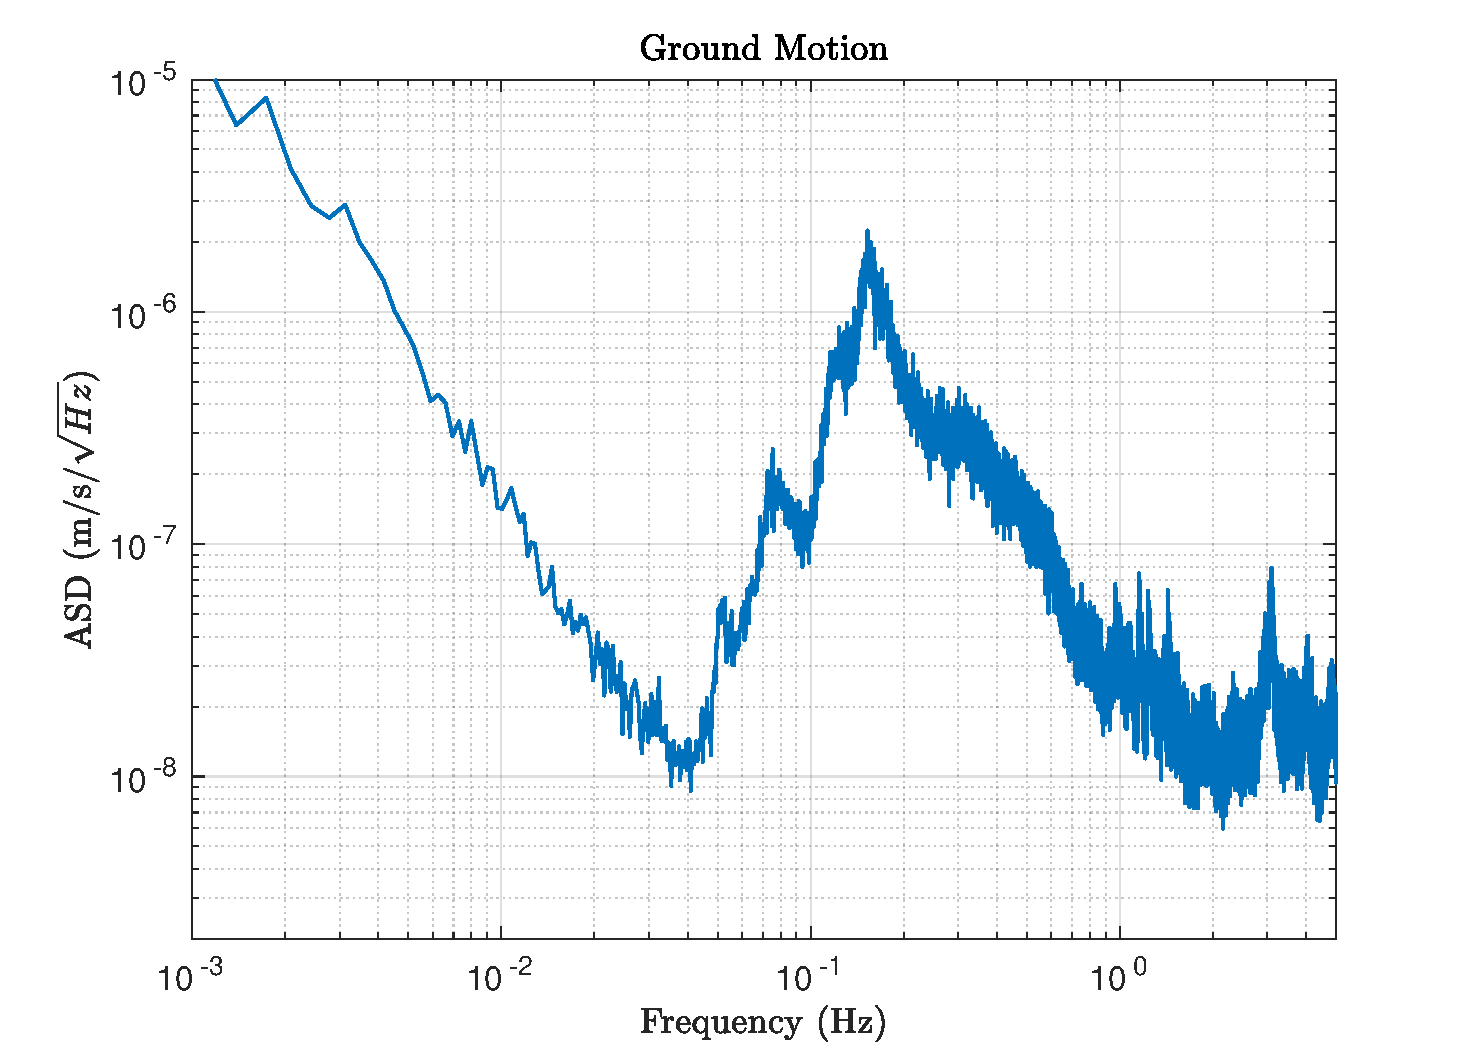
\includegraphics[width=\textwidth]{GroundSpectrum.pdf}
\caption{Amplitude spectral density of typical ground motion as recorded by a horizontal seismometer. \cite{ross2020precision} The spectrum is dominated by anthropengic motion above 1 Hz and the microseism between 30 mHz - 1 Hz. Below 30 mHz the spectrum is dominated by ground rotations caused by the atmosphere.}\label{groundSpec}
\end{centering}
\end{figure}

In addition to the persistent ground motion, there are many sources of large, short-duration motion. The most obvious case is earthquakes but humans also cause such transient with construction activity, explosions (both for mining and weapons testing), etc. The motion caused by these events can be much larger than the spectrum shown in Figure \ref{groundSpec}. However, since these events are transient, many experiments are just paused until the motion stops. As long as the apparatus is not damaged than this only amounts to a loss of data taking time which is acceptable in many circumstances.

The source of ground motion is not necessarily important for torsion balance experiments however, the apparatus must be isolated from this motion in order to achieve high sensitivity. Without isolation, ground motion would swamp any measurement and in many cases make the apparatus not function at all. There are a many methods to isolate from this motion but they broadly fit into two categories: active isolation and passive isolation. 

Active isolation is the process of sensing either the ground motion or the motion of the apparatus and counteracting these motions with some sort of actuator. A system which senses ground motion is called a ``feed-forward'' system because the apparatus is moved based on what is expected to happen, whereas sensing the apparatus motion is called a ``feed-back'' system because the applied motion is based on what has already happened. The exact development of active isolation system falls under the study of control system which has an extensive history and literature from a wide range of fields. Typically these active systems can perform superbly but are limited by the quality of sensors and actuators that are deployed and cost a large sum of both money and development time. 

Passive isolation systems on the other hand tend to be simple in their design. A passive system uses the dynamics of mechanical systems to isolate from motion. Classical examples of these systems are placing the apparatus on rubber or springs and hanging the apparatus from a pendulum. This causes the apparatus to become a oscillator system which has a response function like those shown in Figure \ref{respPlot}. Above the resonant frequency of the system, the motion of the apparatus is decreased by a factor of $\sim (\omega_0/\omega)^2$ where $\omega_0$ is the resonant frequency of the system and $\omega$ is the frequency of motion. If multiple passive systems are stacked than the motion is decreased by $\sim (\omega_0/\omega)^{2N}$ where $N$ is the number of systems.

Torsion balances are inherently passive isolation systems. The dynamics of the swing degree of freedom, Section \ref{swing}, passively isolated the pendulum from horizontal motion. With the addition of a vertical spring at the suspension point, experimenters can also passively isolate from vertical motion. Historically, the combination of the inherent horizontal isolation and a vertical spring achieved sufficient isolation to make seismic motion subdominant except during abnormal conditions (earthquakes, construction nearby, etc.). 

Many extremely sensitivity apparatus today are employing multiple layers of both active and passive seismic isolation. For example, the LIGO gravitational wave observatories deploy three layers of active isolation and four layers of passive in the form of a quadruple pendulum. How much and which types of isolation is up to the experimenter to decide while designing an apparatus based on the frequency of interest and the necessary sensitivity of the instrument.

\section{Electrostatic Couplings}\label{elect}
\section{Magnetic Noise}
\section{Gas Damping} \label{gas}
\section{Gravity Gradients}\label{gravGrad}

\chapter{Data Analysis Techniques}
\section{Fourier Analysis}
\section{Linear Least-Squares Fitting}

\bibliographystyle{unsrt}
\bibliography{TorsionBalances}

\end{document}
